%! suppress = FileNotFound
\documentclass[a4paper,12pt]{report}
\usepackage{graphicx}
\usepackage{hyperref}
\usepackage{float}
\usepackage{makecell}
\usepackage[nottoc]{tocbibind}
\usepackage{biblatex}

\pagestyle{headings}
\graphicspath{{./Images/}}
\hypersetup{
	colorlinks=true,
	linkcolor=blue,
	filecolor=magenta,
	urlcolor=cyan,
}


\begin{document}


\begin{titlepage}
	\begin{center}
		\vspace*{1cm}

		\Huge
		\textbf{Design Document - DD}

		\vspace{0.5cm}
		\large
		January 2021

		\vspace{1.5cm}


		\vfill

		
\includegraphics[scale=0.7]{PolimiLogo}

		\vfill


		\normalsize
		\textbf{KONG XIANGYI} \\
		\textbf{\&} \\
		\textbf{ZHANG YUEDONG}

	\end{center}
\end{titlepage}

\tableofcontents


\chapter{INTRODUCTION}\label{ch:introduction}


\section{Purpose}


\section{Scope}


\section{Definitions, Acronyms, Abbreviations}
\subsection{Definitions} \label{subsec:definitions}
\begin{itemize}
	\item Click Customer : The customer has the required technology to access the store.
							I.e a smartphone.
							They can use the customer terminal software.
	\item Brick Customer : The customer doesn't have the required technology to access the store, they have to hand out "tickets" on the spot.
	\item Store Manager : They have to manage the Store System, include the software and hardware.
	\item Ticket: The ticket is a document which contains three key information: QR Code, the estimated departure time, the queue number, and the Store Planned Roadmap.
					To the click customer, it's \textbf{E-ticket} but to the brick customer,it's \textbf{Paper Ticket},and doesn't contain the estimated departure time, and just a General Store Map without the Planned Road.
	\item QR Code : When customer booked a visit, they will received a QR Code.
	\item QR Code Scanned Machine : A hardware, the Click Customer can use this machine scan their QR code.
	\item Tickets Hand-Out Machine : A hardware, the Brick Customer can use it retrieve their Ticket.
	\item Store Planned Roadmap: A store map that includes a finer way which is recommended form Store System.
	\item Digital Counterpart : A hardware, it with show the queue number.
	\item Store Back-End System : A software, as the back-end manages all stuffs.
	\item On-Time Store Data : A dataset that includes the store's on-time date.
	\begin{itemize}
		\item The current queue
		\item The customers in the store
		\item The maximum number of people in the store.
	\end{itemize}
	\item Long-Term Customers: The Click Customer who visited the store more than one time by the CLup mobile application.
\end{itemize}


\subsection{Acronyms}
\begin{itemize}
	\item RASD - Requirement Analysis and Specification Document
	\item DD - Design Document
	\item CLup - Customers Line-up
	\item UI - User Interface
	\item IOS - iPhone OS
	\item PC - Personal Computer
	\item IaaS - Infrastructure as a Service %TODO delete IaaS
	\item CRM - Customer Relationship Management
	\item LAN - Local Area Network
	\item RAPS - Reliable Array of Partitioned Service
	\item RACS - Reliable Array of Cloned Services
\end{itemize}


\subsection{Abbreviations}
\begin{itemize}
	\item %TODO
\end{itemize}


\section{Revision history}


\section{Document Structure}


\chapter{ARCHITECTURAL DESIGN}\label{ch:architectural-design}

In this chapter, we will describe the architectural design of our system.

We will use the Top-down design approach, design the very high-level structure first,
and then gradually work down to detailed decisions about low-level constructs.
Finally, arrive at detailed decisions.\cite{Slides}
Let us start with the High-level components and their interaction.


\section{Overview: High-level components and their interaction}\label{sec:ArchitectureOverview}

We chose \textbf{3-Tiered architecture} with the \textbf{Thin Client} strategy for our system.
As shown in Fig.\ref{fig:ThreeTieredArchitecture}.\cite{SistemiInformativi}

\textbf{Tier-1} is the \textbf{Presentation Layer}.
This layer will deploy the Click Client's Mobile Application,
the Store Manager's Management System,
and even Digital Counterpart and Ticket Hand-Out Machine's presentation.

\textbf{Tier-2} is the \textbf{Logic Application Layer}.
This layer will deploy our Back-End System's components.

\textbf{Tier-3} is the \textbf{Data Access Layer}.
This layer includes our DBMS and the Data Base.

Finally, our high-level architecture is shown in Fig.\ref{fig:HighLevelArchitecture}.
The Store Manager's PC and other hardware will connect with the Ethernet Switch Hub.
The Click Customer's Mobile App will communicate with our Back-End System via the Internet.

More detailed components will be introduced in the next sections.
In particular, in Sec.\ref{sec:deployment-view}.
There, we will introduce the DMZ, load balancer, and other Deployment plan selections.

\begin{figure}
	\centering
	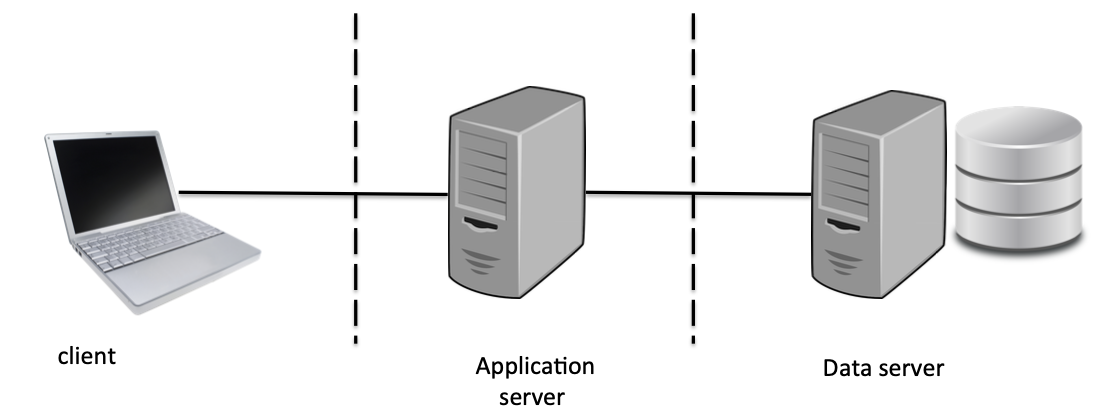
\includegraphics[scale=0.7]{ThreeTiered}
	\caption{3-Tiered architecture}
	\centering
	\label{fig:ThreeTieredArchitecture}
\end{figure}

\begin{figure}
	\centering
	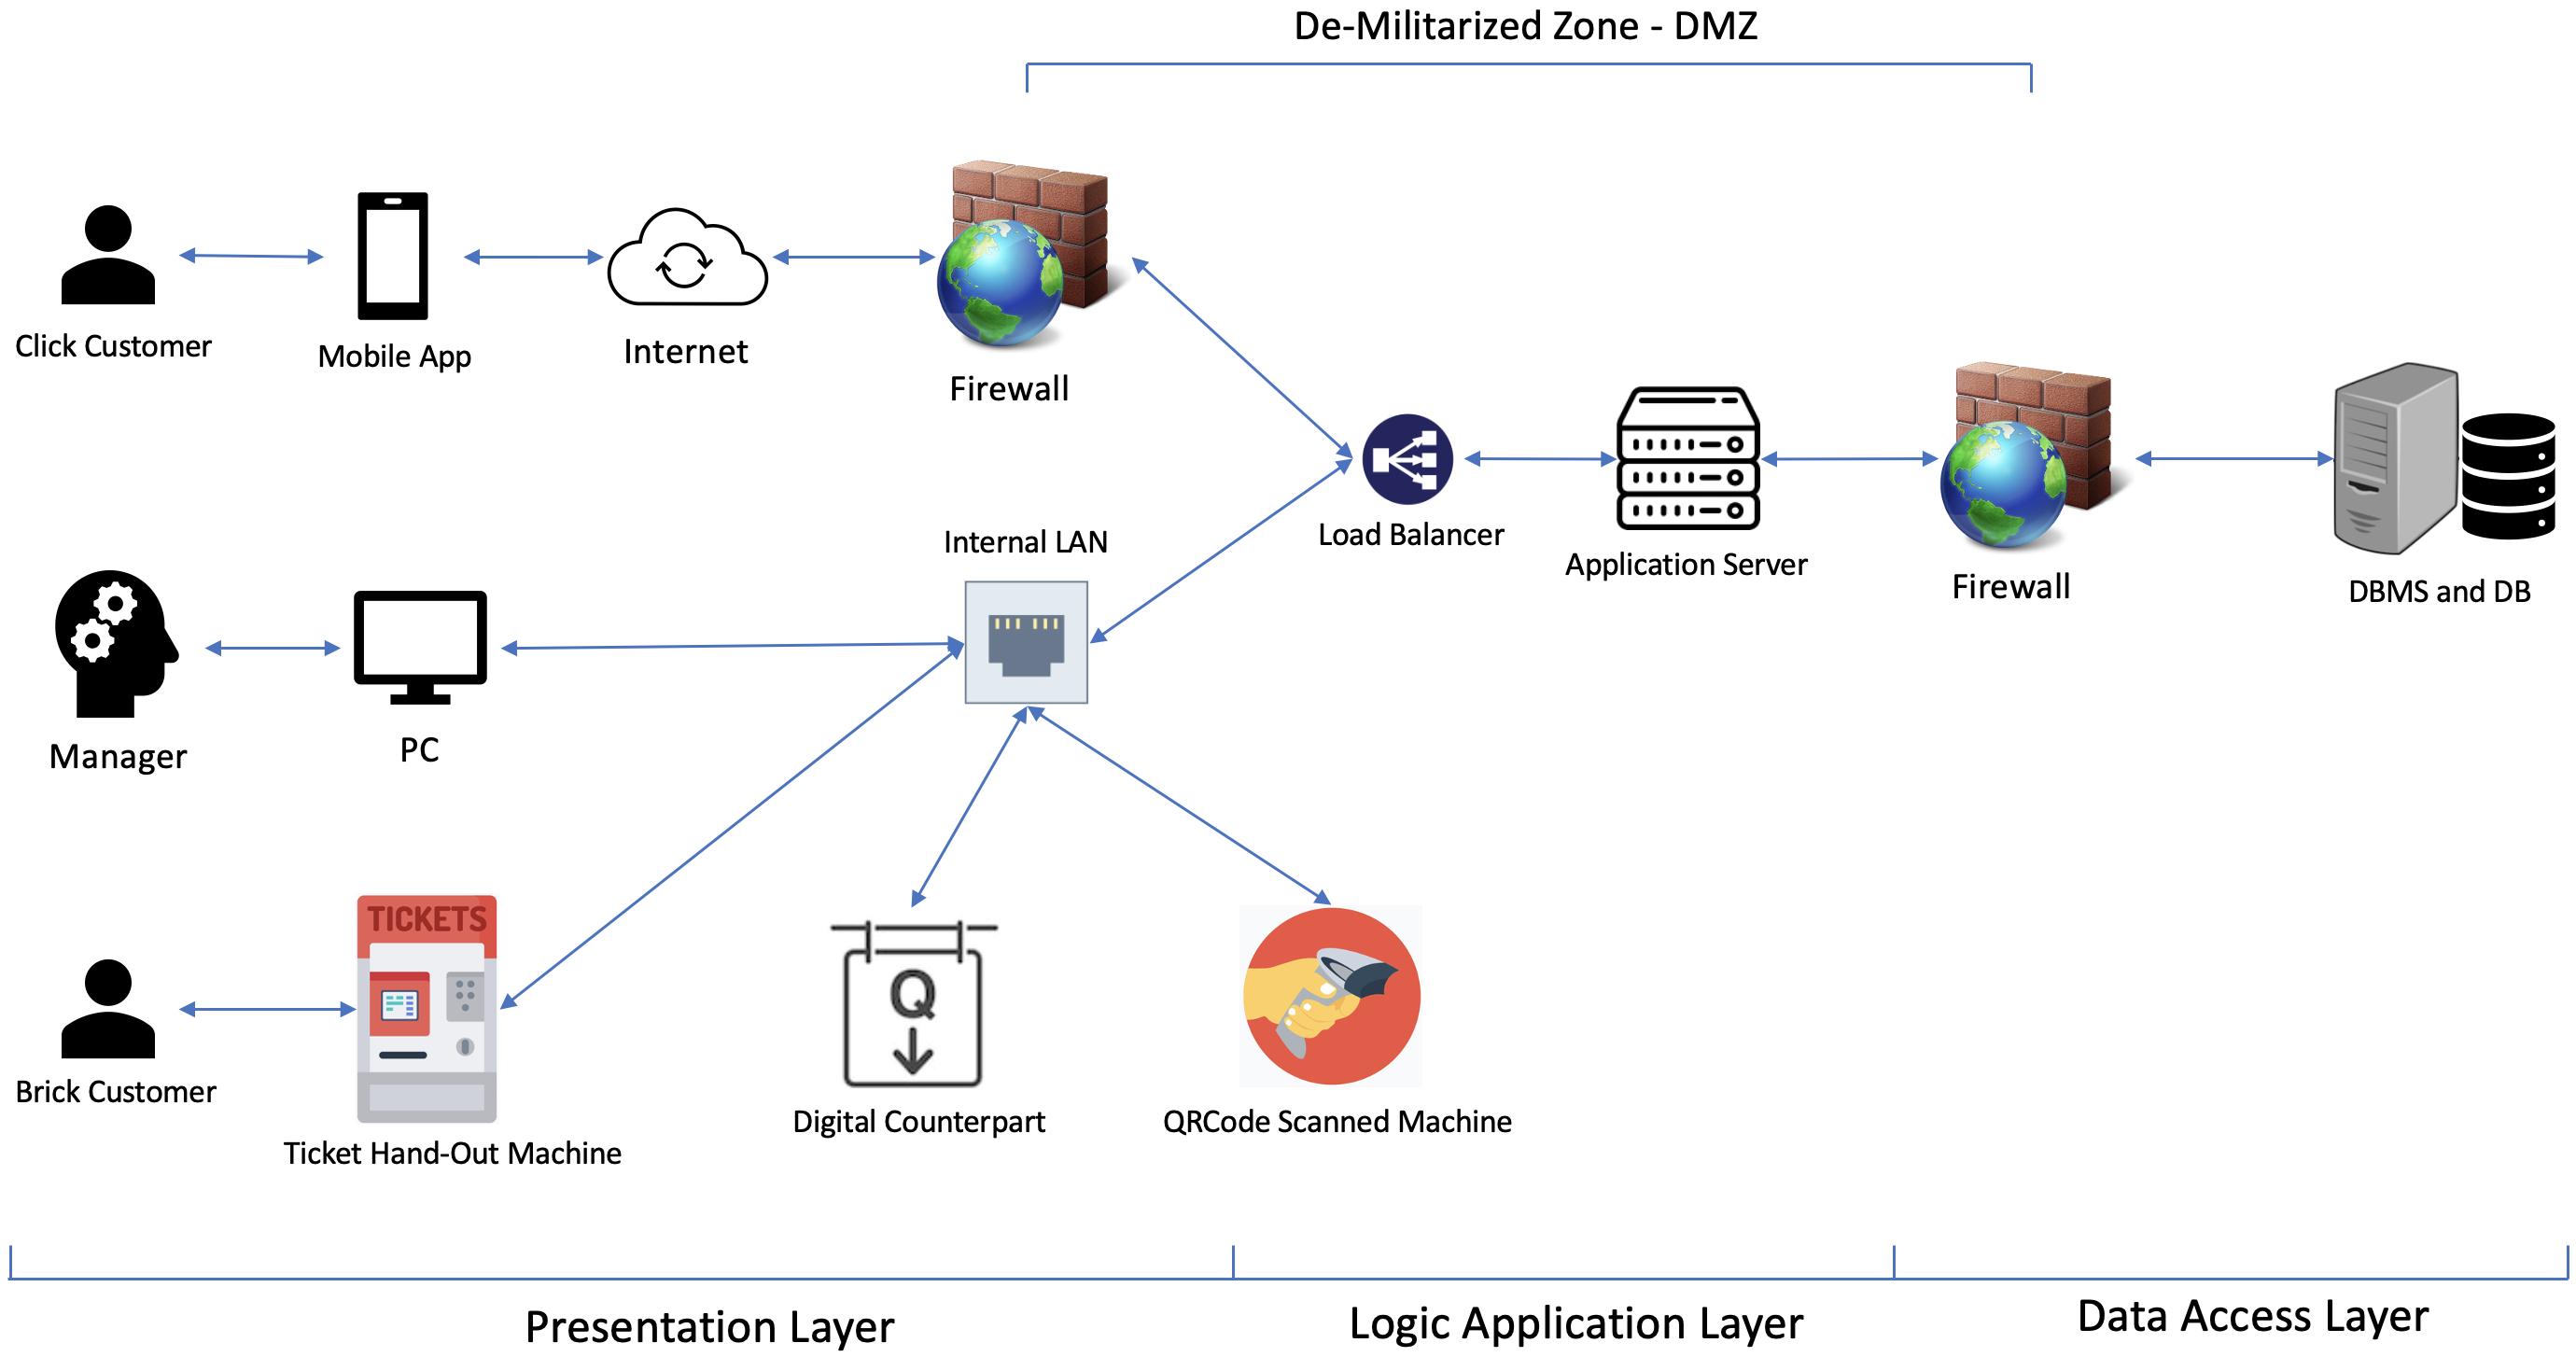
\includegraphics[scale=0.31]{HighLevelArchitecture}
	\caption{High level architecture}
	\centering
	\label{fig:HighLevelArchitecture}
\end{figure}

\section{Component View} \label{sec:ComponentView}
The following diagram Fig.\ref{fig:ComponentDiagram} is the \textbf{Component Diagram}, and it contains all components in our system.
This diagram shows the 3-Tiered Architecture of our system.
The Yellow components are in Presentation Layer.
The blue components are in the Logic Application Layer, and the Green components DBMSServer is in the Data Access Layer.
We will separately introduce all these components in this section, for the interfaces, please go to Sec.\ref{sec:component-interfaces}.

The \textbf{Redirector} component is a bridge for communicating the Presentation Layer and the Logic Application Layer.
It is transparent to User and back-end systems, plays the role of forwarding information on both sides, and connect interfaces.
It has four subsystems, respectively, responsible for communicating with four types of devices, as shown in Fig.\ref{fig:component_diagram_redirector}.

The \textbf{ClickCustomerRedirector} will transfer the message between Mobile Application and the Application Server.
The Register message will pass by the RegisterNewClickCustomer, and look out the Valid/History Booking will use the GetClickCustomerData Interface,
this Interface will return all information of this Customer.
For the most important operation - Booking a visit, use GetBookingSchedule to get the available Time/Date.
Then, through the ModifyClickCustomerData Interface to submit the Booking,
by the way, it also can modify other available data of this Customer.
Moreover, the SendNotifyToClickCustomer Interface will handle Notify message.
The Mobile Application can actively "pull" Notify message through this Interface from the Back-End System.
To "push" Notify information, we will use the Observer Pattern.
It will introduce in Sec.\ref{sec:SelectedArchitecturalStylesAndPatterns}

The \textbf{TicketMachineRedirector} will transfer the Ticket Hand-Out Machine's message.
It needs two pieces of information, the allowed \hyperref[subsec:definitions]{maximum number of people in the store} and how many Customers in the Queue in time.
So The GetQueueSchedule and GetMaxNumberInStore Interface can do these operations, and these two fields will show on the Ticket Machine's screen.
Finally, the retrieve ticket operation will handle by the ModifyQueueSchedule Interface.
It will put a BrickCustomer into the Queue.

The \textbf{DigitalCounterpartRedirector} will help the \hyperref[subsec:definitions]{Digital Counterpart} display the next queue number.
The Customer can enter the store after found his number on the Digital Counterpart.

The \textbf{ManagementSystemRedirector} will function for the Management System of our Store Manager.
This redirector will transmit the message between the Presentation layer's web page and the Back-End System.
Through the Interface shown in Fig.\ref{fig:component_diagram_RedirectoSubsystem}, the Manager can realize his operation like reschedule someone's Booking, adjust the Queue order, or lower the maximum number.

The next three subsystems are the core subsystems in our application layer.

The \textbf{CRM} component is responsible for communicating with Click Customers' End, handle the register, Log-In, Booking, data-send, and notify-send operation.
The Booking operation will communicate with the Booking Schedule component, send the Booking Information, general E-Ticket, and store all data in the database.
In addition, it must also help the Customer calculate the estimated departure time from depart place to the store, so it will call the GoogleMap API to query it.

The \textbf{Booking Schedule} component is working for all Booking tasks.
Receive the Booking from CRM, handle the Store Manager's modified Booking, send the Booking schedule to the Queue Schedule component, and store all Booking Schedule to the database.

The \textbf{Queue Schedule} subsystem is the main component to communicate with the Store Manager's Management System.
It has to take the Booking schedule to calculate the Queue order and handle the Store Manager's modification for the Maximum value or Queue order.

At last, the \textbf{Database System}, it will manage all database, and handle the CRM, BookingSchedule, QueueSchedule's Query/Insert/Update.


\begin{figure}
	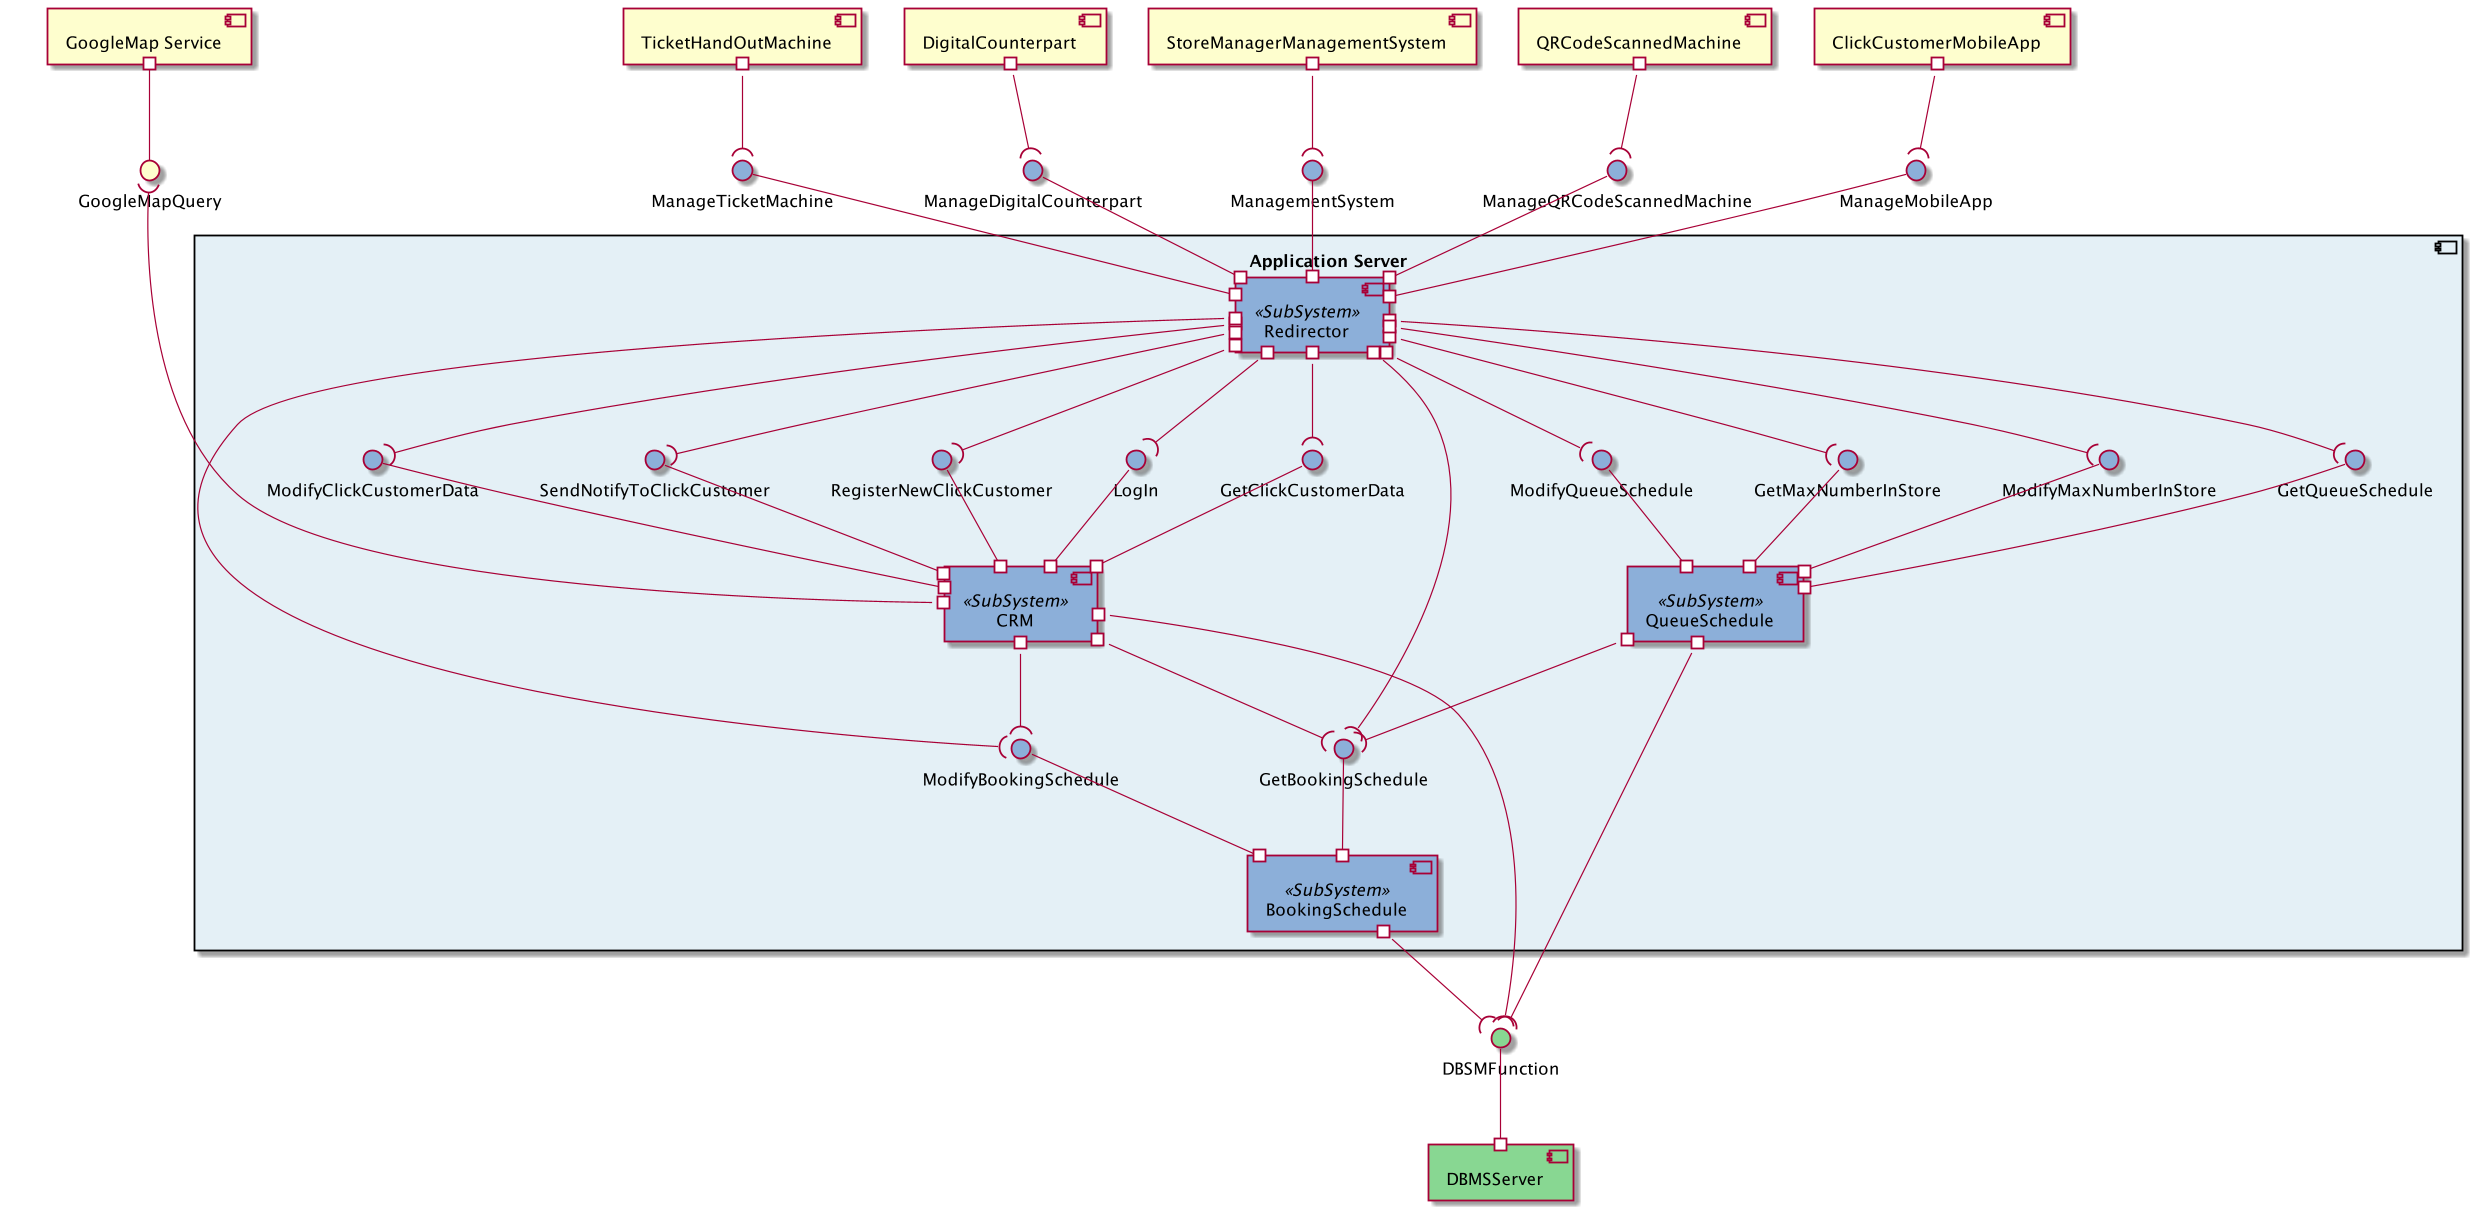
\includegraphics[width=1.25\textwidth]{component_diagram}
	\centering
	\caption{Component Diagram}
	\label{fig:ComponentDiagram}
\end{figure}

\begin{figure}
	\centering
	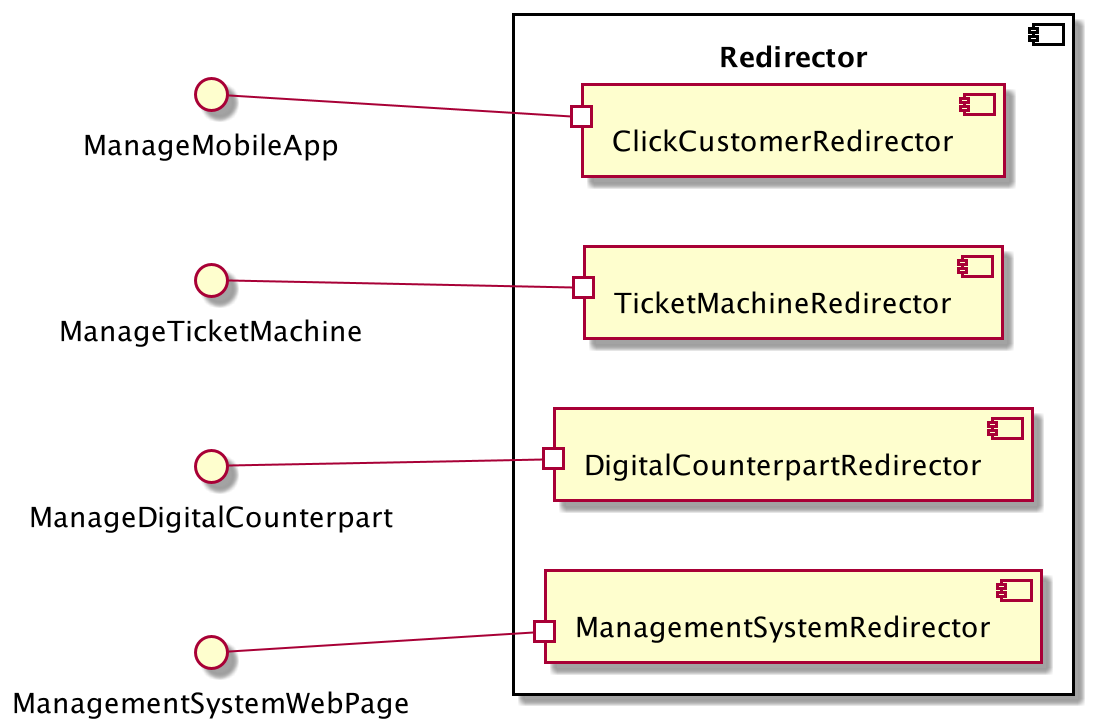
\includegraphics[scale=0.2]{component_diagram_redirector}
	\caption{Redirector Component Diagram}
	\centering
	\label{fig:component_diagram_redirector}
\end{figure}

\begin{figure}
	\centering
	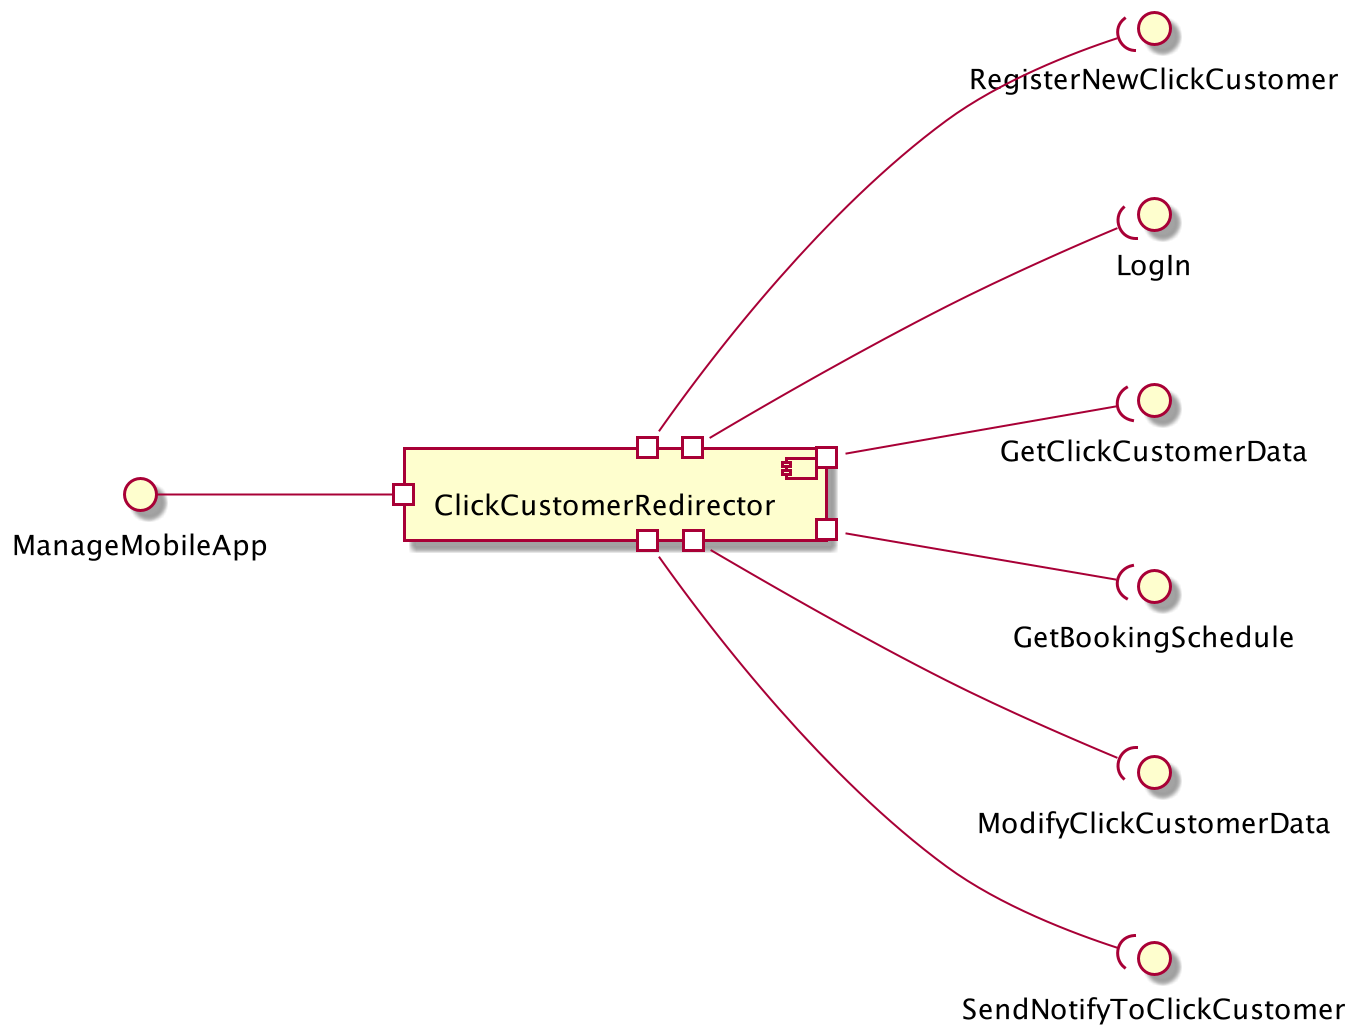
\includegraphics[scale=0.2]{component_diagram_ClickCustomerRedirector}
	\vspace{10mm}
	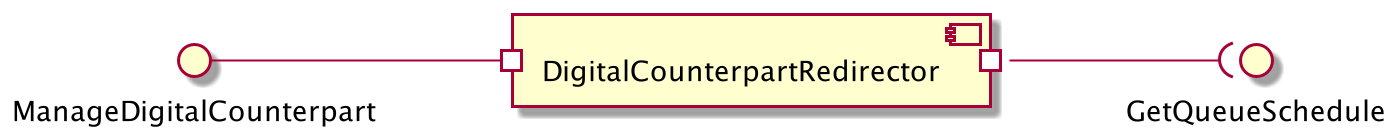
\includegraphics[scale=0.2]{component_diagram_DigitalCounterpartRedirector}
	\vspace{10mm}
	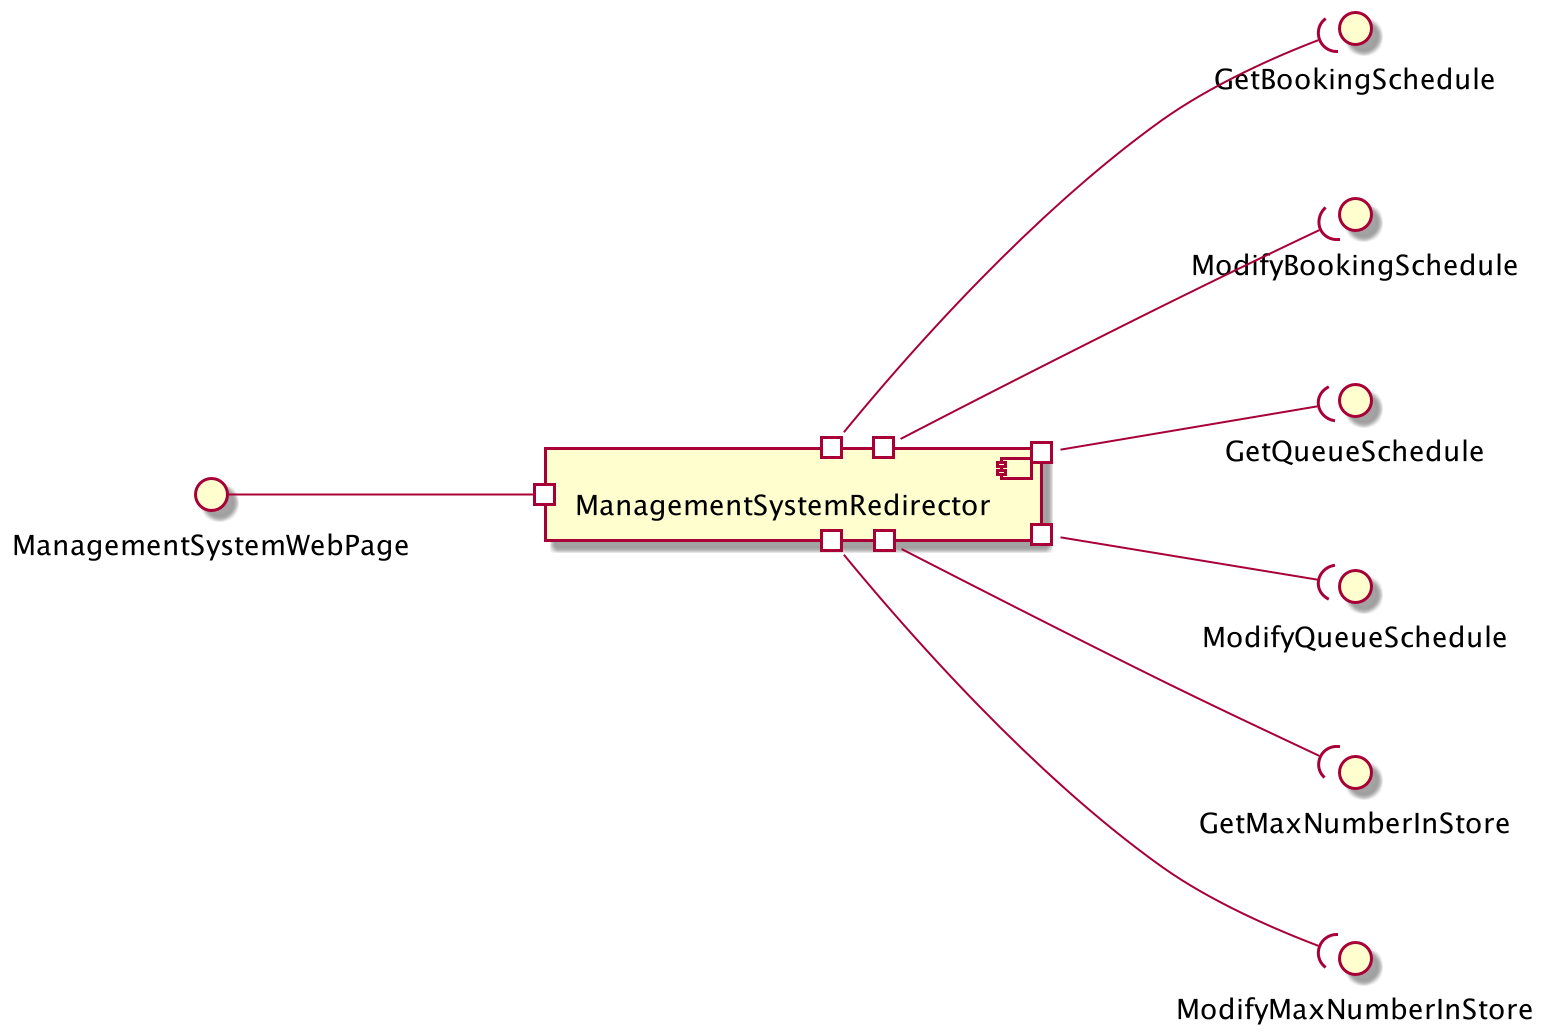
\includegraphics[scale=0.2]{component_diagram_ManagementSystemRedirector}
	\vspace{10mm}
	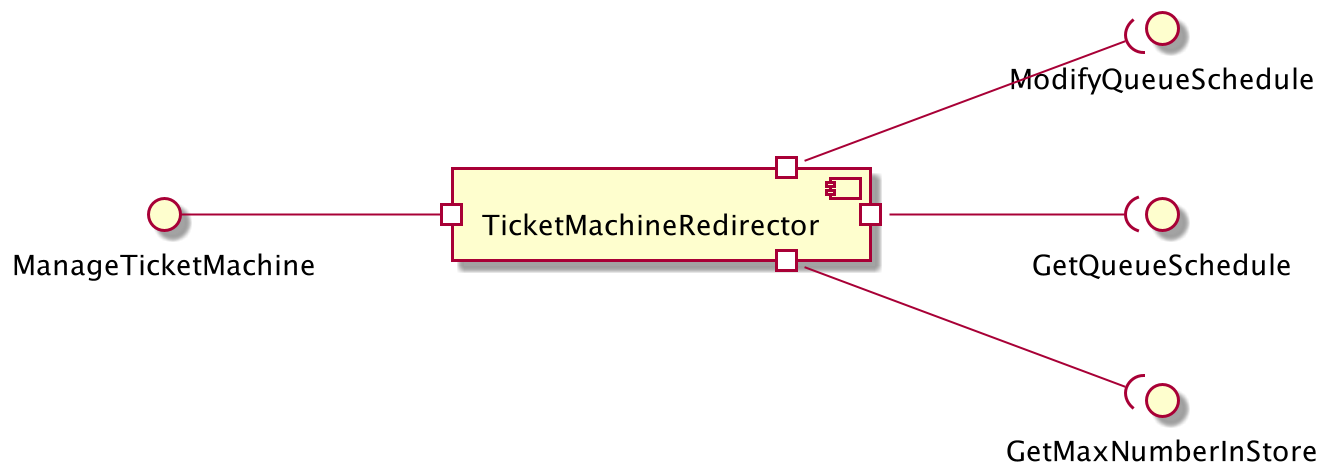
\includegraphics[scale=0.2]{component_diagram_TicketMachineRedirector}
	\vspace{10mm}
	\caption{Redirector's Subsystem Component Diagram}
	\centering
	\label{fig:component_diagram_RedirectoSubsystem}
\end{figure}


\section{Deployment View}\label{sec:deployment-view}

Our deployment situation, as shown in Fig.\ref{fig:deployment_diagram}.
Three colors respectively represent the three layers.
The Green devices are in the Data Access Layer, the Blue devices are in the Logic Application Layer,
and the Yellow devices are in the Presentation Layer.

For all our devices, to reduce the development/management/maintenance cost,
we will use the same Operation System - Ubuntu 20.10, and run in the same Runtime Environment - Java SE Runtime Environment 8u271.

In the \textbf{Presentation Layer}, The Store Manager's PC, the Digital Counterpart, and the Ticket Machine are the Internal Devices, which means we must manage them ourselves.
We built a LAN to connecting them with the Application Server via the Switch Hub. In our LAN, we used the Ethernet Protocol.
Moreover, we have chosen the Thin Client strategy in the system architecture, so all our Internal Devices can run on the Raspberry Pi 4.
It is a very low-cost deployment solution.

In contrast, the Mobile Application is the External Device that will run on the Click Customer's SmartPhone.
It has to connect with Back-End System via the Internet.
We will separately develop the Client End for the two kinds of systems - IOS and Andriod System.

In the \textbf{Application Layer}, We refer to the network security part of the information system book P.243.
We used two Firewalls to build a \textbf{DeMilitarized Zone - DMZ}.
The external network can only access the resources exposed in the DMZ (Our Application API), and the rest of the network is behind the second firewall.
The DMZ functions as an isolated subnet between the Internet and the private network,
So that our database can be better protected.\cite{SistemiInformativi}

For the \textbf{Load Balancer}, we must first ensure that our Internal Devices can allocate enough Server resources and then ensure the Click Customer's resources, so we considered two plans.
\begin{enumerate}
	\item Allocate dedicated Application Servers for our Internal Device, and other Application Servers connect with Load Balancer.
	\item Do not allocate server resources separately for internal devices, but set higher weights for Internal Devices in the load balancer.
\end{enumerate}
Plan 1 can guarantee that our system's most important part can work well, whether the balancer is working or how crowded the network is.
Plan 2 ensures that when some servers are not working, the well-function servers can always allocate to Internal Devices.
After weighing, we finally chose plan 2.
Because we think Plan 2 has higher system availability/maintainability.

As mentioned above, for the \textbf{Application Server}, we adopted the Reliable Array of Cloned Services - RACS, like the figure in the Information System Book P.202\cite{SistemiInformativi}, Fig.\ref{fig:RACS}.
The load balancer must allocate the higher weights to Internal Devices, and all our Application Server will run the same application.
There is a different point in our case from the figure: we have separated the database and the Application Server.
Nevertheless, cause our business is "write-intensive", so we used the shared-disk configuration in essence.

Finally, the \textbf{Database system}, we selected PostgreSQL as the Database Management System cause it is Open Sources and stable.
Then we will use the relational database to implement it.
For Security, as the DMZ mentioned above, only our private network can access this system, so that the external network will difficultly attack our database.


\begin{figure}
	\centering
	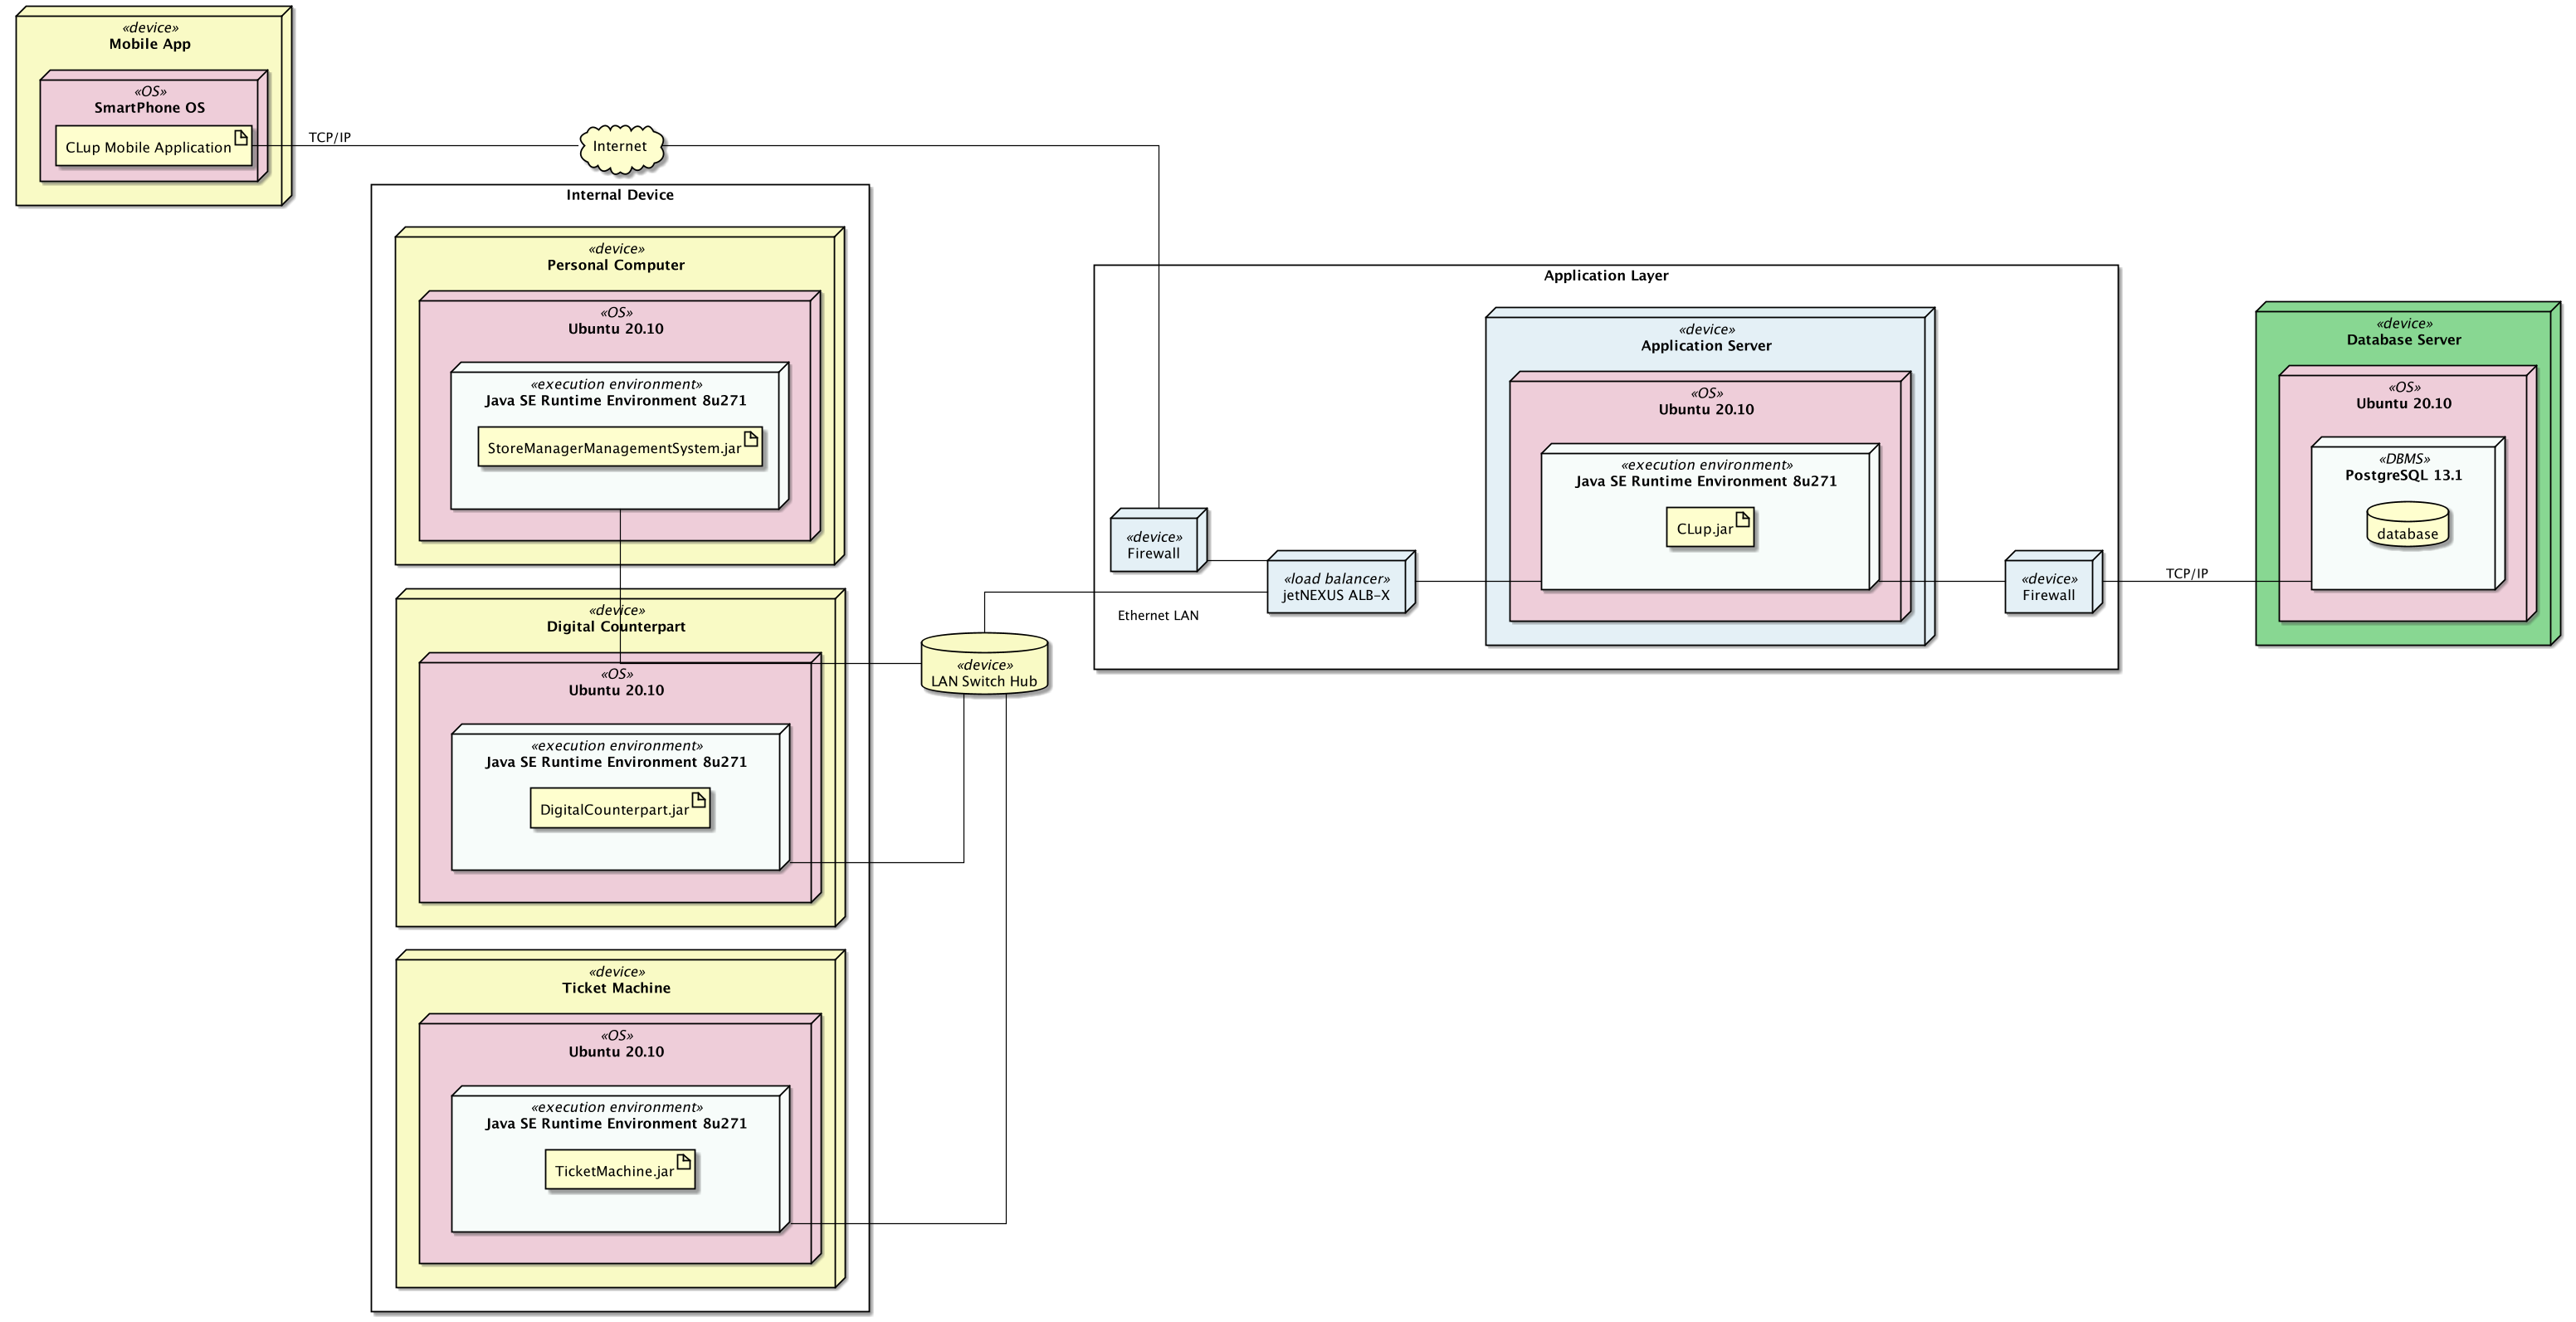
\includegraphics[width=1.25\textwidth]{deployment_diagram}
	\caption{Deployment Diagram}
	\centering
	\label{fig:deployment_diagram}
\end{figure}

\begin{figure}
	\centering
	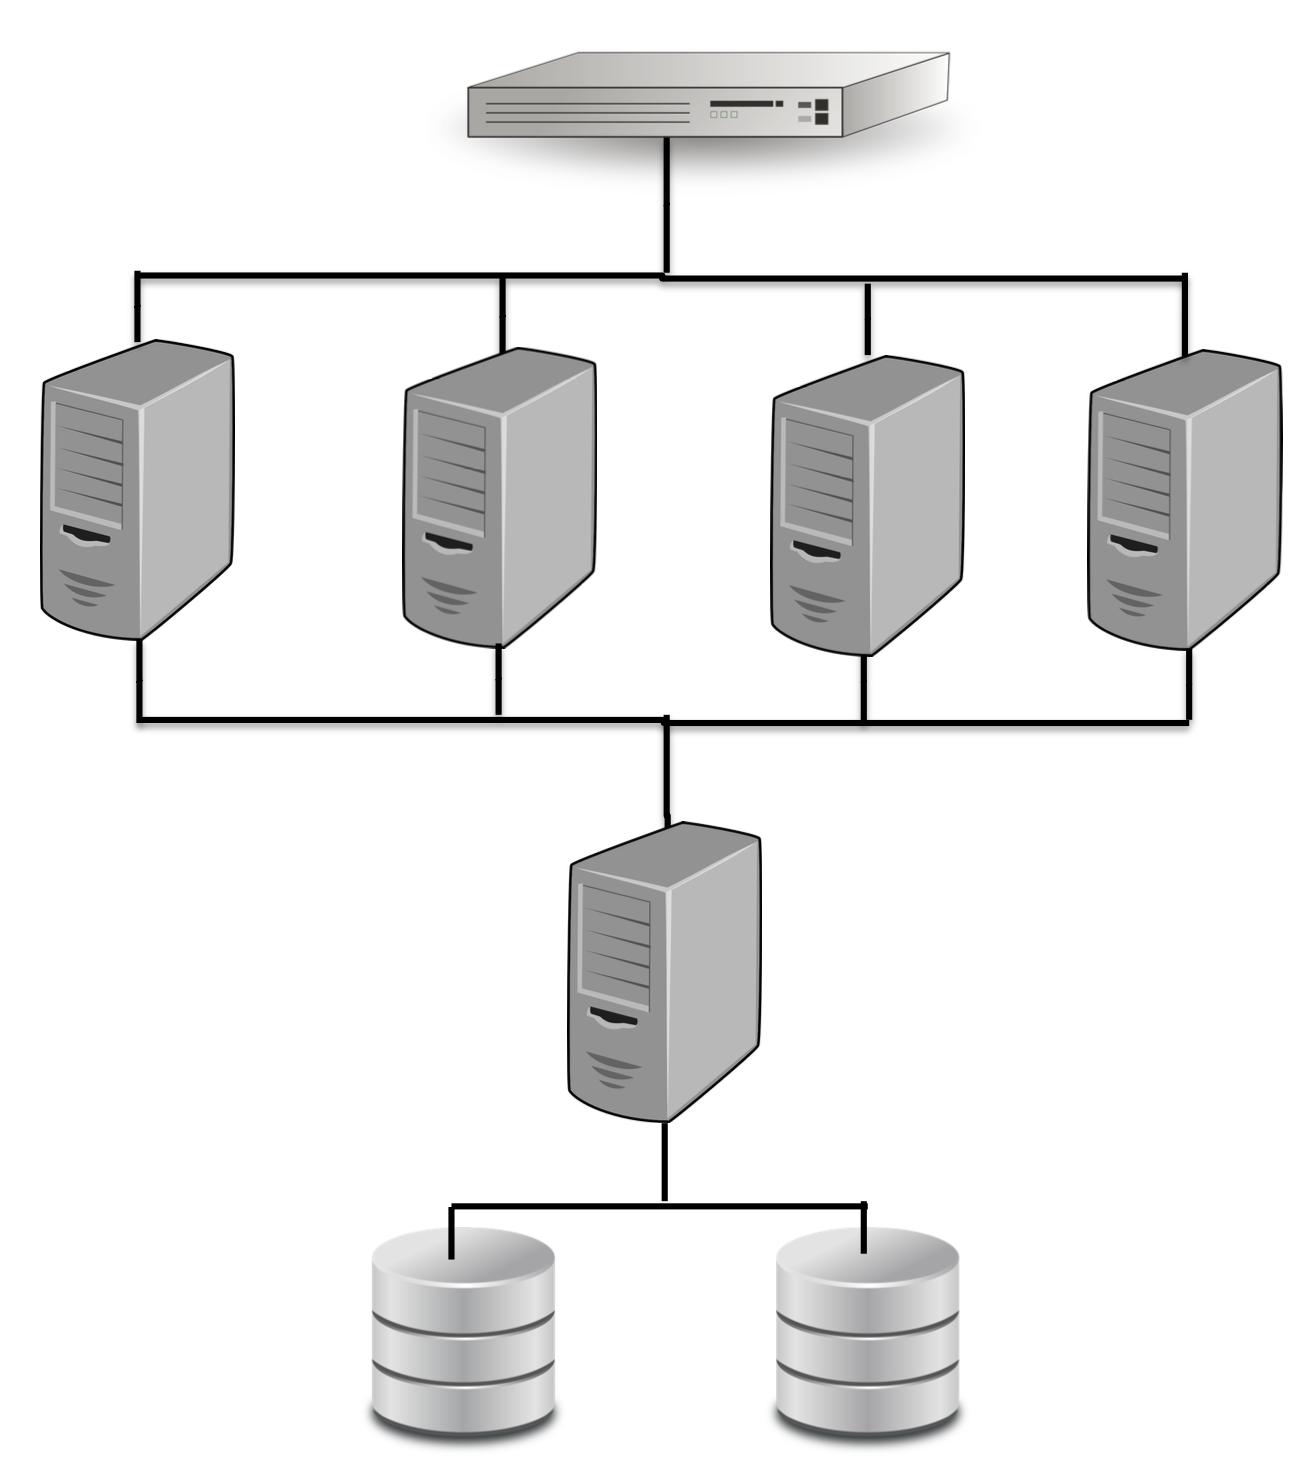
\includegraphics[width=0.5\textwidth]{RACS}
	\caption{RACS: Shared-disk o cluster Configuration}
	\centering
	\label{fig:RACS}
\end{figure}


\section{Runtime View}



\section{Component Interfaces}\label{sec:component-interfaces}


\section{Selected Architectural Styles and Patterns}\label{sec:SelectedArchitecturalStylesAndPatterns}

%MVC
%Observer Pattern

\section{Other Design Decisions}

\chapter{USER INTERFACE DESIGN}\label{ch:user-interface-design}


\chapter{REQUIREMENTS TRACEABILITY}\label{ch:requirements-traceability}


\chapter{IMPLEMENTATION, INTEGRATION AND TEST PLAN}\label{ch:implementation-integration-and-test-plan}


\chapter{Effort Spent}

\begin{itemize}
	\item \textbf{Kong XiangYi}
	\begin{center}
		\scalebox{0.8}{
			\begin{tabular}{ |c|c|c| }
				\hline
				Date & Task & Hours \\
				\hline
				\hline
				2021/01/02 & Group discussion and task assignment & 2h \\
				\hline

		\end{tabular}}
	\end{center}


	\item \textbf{Zhang YueDong}
	\begin{center}
		\scalebox{0.8}{
			\begin{tabular}{ |c|c|c| }
				\hline
				Date & Task & Hours \\
				\hline
				\hline
				2021/01/01 &  Launch DD  & 2h \\
				\hline
				2021/01/02 & Group discussion and task assignment & 2h \\
				\hline
				2021/01/03 & Did S.\ref{ch:architectural-design}.\ref{sec:ArchitectureOverview}
				and S.\ref{ch:architectural-design}.\ref{sec:ComponentView}
				Component Diagram & 3h \\
				\hline
				2021/01/04 & Did S.\ref{sec:ComponentView}.
				Component Diagram describe. & 2h \\
				\hline
				2021/01/05 & Did S.\ref{sec:deployment-view}.
				Deployment Diagram and describe. & 5h \\
				\hline
			\end{tabular}}
	\end{center}
\end{itemize}




%Bibliographic references
\begin{thebibliography}{9}

\bibitem{SistemiInformativi}
Cinzia Cappiello, Mariagrazia Fugini, Paul Grefen, Barbara Pernici, Pierluigi Plebani, Monica Vitali. (7 settembre 2018)  Fondamenti di Sistemi informativi: per il Settore dell'Informazione.

\bibitem{IEEESDD}
"IEEE Standard for Information Technology--Systems Design--Software Design Descriptions," in IEEE STD 1016-2009 , vol., no., pp.1-35, 20 July 2009, doi: 10.1109/IEEESTD.2009.5167255.

\bibitem{IEEEAD}
"ISO/IEC/IEEE Systems and software engineering -- Architecture description," in ISO/IEC/IEEE 42010:2011(E) (Revision of ISO/IEC 42010:2007 and IEEE Std 1471-2000) , vol., no., pp.1-46, 1 Dec.
2011, doi: 10.1109/IEEESTD.2011.6129467.

\bibitem{Slides}
Elisabetta Di Nitto, Matteo Rossi. (A.Y.2020/2021) The slides of the Software Engineering 2 course.

\end{thebibliography}


\end{document}

